\documentclass[conference]{IEEEtran}
% The following line is only needed to identify funding in the first footnote. If that is unneeded, please comment it out.
\usepackage{amsmath,amssymb,amsfonts}
\usepackage{algorithmic}
\usepackage{graphicx}
\usepackage{textcomp}
\usepackage{xcolor}
\usepackage{float}

\floatstyle{boxed} 
\restylefloat{figure}

\def\BibTeX{{\rm B\kern-.05em{\sc i\kern-.025em b}\kern-.08em
    T\kern-.1667em\lower.7ex\hbox{E}\kern-.125emX}}
\begin{document}

\title{Workshop 2: System Design for Detecting Sleep States Using Accelerometers}
\title{\IEEEoverridecommandlockouts Workshop 2: System Design for Detecting Sleep States Using Accelerometers}
\author{
	\IEEEauthorblockN{Juan Carlos Quintero Rubiano}
	\IEEEauthorblockA{Code: 20232020172\\
		\textit{Systems Engineering} \\
		\textit{Francisco Jose de Caldas District University}\\
		Bogota, Colombia \\
		jcquineror@udistrital.edu.co}\\
	\IEEEauthorblockN{Juan Felipe Wilches Gomez}
	\IEEEauthorblockA{Code: 20231020137\\
		\textit{Systems Engineering} \\
		\textit{Francisco Jose de Caldas District University}\\
		Bogota, Colombia \\
		jfwilchesg@udistrital.edu.co}
	\and
	\IEEEauthorblockN{Juan Nicolas Diaz Salamanca}
	\IEEEauthorblockA{Code: 20232020059\\
		\textit{Systems Engineering} \\
		\textit{Francisco Jose de Caldas District University}\\
		Bogota, Colombia \\
		jndiazs@udistrital.edu.co}
}

\maketitle

\begin{abstract}
	This document builds upon the systemic analysis conducted in Workshop 1 for the Kaggle competition "Child Mind Institute - Detect Sleep States." The focus is on designing a robust system to detect sleep states using accelerometer data. Key findings from the previous analysis, including constraints, data characteristics, and chaos-theory factors, are summarized to guide the design process. The proposed design aims to address identified weaknesses and optimize system performance.
\end{abstract}

\begin{IEEEkeywords}
	System design, sleep state detection, accelerometers, chaos theory, optimization.
\end{IEEEkeywords}

\section{Introduction}
\subsection{Overview of Workshop 1 Findings}
The systemic analysis conducted in Workshop 1 provided a comprehensive understanding of the system for detecting sleep states using accelerometer data. The following key findings were identified:

\begin{itemize}
	\item \textbf{Constraints:}
	      \begin{itemize}
		      \item Sleep periods must be at least 30 minutes long, with interruptions no longer than 30 minutes.
		      \item Only the longest sleep window per night is recorded.
		      \item Device removal periods are not annotated, introducing potential gaps in data.
	      \end{itemize}
	\item \textbf{Data Characteristics:}
	      \begin{itemize}
		      \item The dataset includes accelerometer data with features such as \texttt{anglez} and \texttt{enmo}, which are critical for detecting sleep states, and a \texttt{timestamp} column for time-based analysis.
		      \item Labels for sleep onset and wake events are provided, enabling supervised learning approaches.
	      \end{itemize}
	\item \textbf{Chaos-Theory Factors:}
	      \begin{itemize}
		      \item Sensitivity to initial conditions: Small variations in accelerometer data can lead to significant changes in sleep state classification.
		      \item Randomness in sleep patterns: External factors such as environmental conditions and individual differences introduce unpredictability.
	      \end{itemize}
\end{itemize}

\subsection{Insights from Systemic Analysis}
The systemic analysis provided the following critical insights for designing the system:

\begin{itemize}
	\item \textbf{Feature Importance:}
	      \begin{itemize}
		      \item The accelerometer features \texttt{anglez} and \texttt{enmo} are pivotal for detecting sleep states. Proper preprocessing, such as normalization and noise filtering, is essential to maximize their utility.
		      \item The \texttt{timestamp} column enables time-series analysis, which is crucial for capturing temporal dependencies in sleep patterns.
	      \end{itemize}

	\item \textbf{Handling Data Gaps:}
	      \begin{itemize}
		      \item Device removal periods and unannotated gaps in the data introduce missing values that require robust imputation techniques or strategies to handle incomplete data effectively.
		      \item Strategies such as forward-filling, interpolation, or machine learning-based imputation can be explored to address these gaps.
	      \end{itemize}

	\item \textbf{Temporal Dependencies:}
	      \begin{itemize}
		      \item Sleep states are inherently sequential and time-dependent. Leveraging models designed for time-series data, such as Long Short-Term Memory (LSTM) networks or Temporal Convolutional Networks (TCNs), can improve classification accuracy.
		      \item Capturing transitions between sleep and wake states is critical for accurate predictions.
	      \end{itemize}

	\item \textbf{Model Robustness:}
	      \begin{itemize}
		      \item The system must account for sensitivity to initial conditions, as small variations in accelerometer data can lead to significant changes in classification outcomes.
		      \item Randomness in sleep patterns, influenced by external factors such as environmental conditions or individual variability, requires the model to generalize well across diverse scenarios.
		      \item Techniques such as data augmentation, ensemble modeling, and robust validation can help improve model reliability.
	      \end{itemize}

	\item \textbf{Optimization Goals:}
	      \begin{itemize}
		      \item The design should focus on minimizing false positives (e.g., misclassifying wake states as sleep) and false negatives (e.g., missing sleep onset events) to ensure high precision and recall.
		      \item Computational efficiency is critical, especially if the system is intended for real-time or large-scale deployment.
	      \end{itemize}
\end{itemize}

\section{Requirements Definition}

Based on the initial analysis and the context of the Kaggle competition "Child Mind Institute - Detect Sleep States", the following requirements have been identified for the system design.

\subsection{Translation of Analysis Findings into Design Requirements}

The findings from the systemic analysis are translated into concrete design requirements, covering both functional and non-functional aspects.

\subsubsection{Functional Requirements}
\begin{itemize}
	\item \textbf{Sleep State Detection:} The system must accurately detect sleep and wake states from accelerometer data.
	\item \textbf{Segregation of Longest Sleep Periods:} The system must identify and segregate the longest sleep periods, which must be at least 30 minutes long, as explained in the constraints.
	\item \textbf{Event Annotation:} The system must identify and annotate sleep onset and wake events.
	\item \textbf{Data Gap Handling:} The system should handle missing or incomplete data due to device removal or recording gaps.
\end{itemize}

\subsubsection{Non-Functional Requirements}
\begin{itemize}
	\item \textbf{Performance:} The system should process data with low latency (e.g., response time under 1 second for real-time use) and handle large volumes of time-series data efficiently.
	\item \textbf{Reliability:} The system must achieve high accuracy in sleep state classification (e.g., precision and recall above 90\%) and tolerate occasional data loss or noise.
	\item \textbf{Scalability:} The architecture should allow for scaling to accommodate more users or increased data volume without significant performance degradation.
	\item \textbf{Interpretability:} The system should provide transparent and understandable explanations for its predictions to support clinical and research decision-making.
	\item \textbf{Privacy and Ethics:} The system must ensure data privacy and comply with relevant regulations (e.g., GDPR), especially considering the sensitive nature of children's health data.
	\item \textbf{Adaptability:} The system should be flexible to support studies in different environments and populations, enabling personalized interventions.
\end{itemize}

\subsubsection{Requirements Prioritization}
Requirements are classified as follows:
\begin{itemize}
    \item \textbf{Essential:} Sleep state detection, real-time processing, high accuracy, data privacy.
    \item \textbf{Desirable:} Advanced data gap handling, scalability for large-scale deployment.
    \item \textbf{Optional:} Integration with external health platforms, customizable alerting features.
\end{itemize}

\subsubsection{Requirements Documentation}
All functional and non-functional requirements are documented in a clear and measurable way to ensure they are verifiable during system validation.
\paragraph{Functional Requirements Verification}
\begin{itemize}
    \item \textbf{Sleep State Detection:} Accuracy will be measured using metrics such as precision, recall, and F1-score. The system must achieve at least 90\% precision and recall on a validation dataset.
    \item \textbf{Segregation of Longest Sleep Periods:} The system will be tested on a dataset with annotated sleep periods. It must correctly identify and segregate the longest sleep period in at least 95\% of cases.
    \item \textbf{Event Annotation:} The system's ability to annotate sleep onset and wake events will be evaluated against ground truth labels. A minimum accuracy of 90\% is required.
    \item \textbf{Data Gap Handling:} The system will be tested with datasets containing simulated gaps. It must impute or handle missing data without reducing classification accuracy below 85\%.
    \item \textbf{Event Detection AP Metric:} The system will be evaluated using the competition's Average Precision (AP) metric for event detection. It must achieve a high AP score by accurately matching predicted events to ground-truth events within the specified tolerance thresholds.
\end{itemize}

\paragraph{Non-Functional Requirements Verification}
\begin{itemize}
    \item \textbf{Performance:} The system's processing time will be measured. It must process data with a response time under 1 second for real-time use and handle datasets of up to 1 million rows without significant performance degradation. Additionally, the system must comply with competition constraints, ensuring that CPU or GPU notebooks complete execution within 9 hours.
    \item \textbf{Reliability:} The system will undergo stress testing with noisy and incomplete datasets. It must maintain classification accuracy above 75\% under these conditions.
    \item \textbf{Scalability:} The system will be deployed in a simulated environment with increasing user loads. It must scale to support at least 1,000 concurrent users without exceeding a 5\% increase in response time.
    \item \textbf{Interpretability:} The system will be evaluated by domain experts for its ability to provide clear and understandable explanations for predictions. At least 80\% of experts must rate the explanations as satisfactory or better.
    \item \textbf{Privacy and Ethics:} Compliance with GDPR and other relevant regulations will be verified through an audit. The system must pass all privacy and security checks.
    \item \textbf{Adaptability:} The system will be tested with datasets from different populations and environments. It must maintain accuracy above 85\% across all scenarios.
    \item \textbf{Submission Compliance:} The system must generate a submission file named \texttt{submission.csv} that adheres to the competition's requirements. The notebook must run without internet access and use only freely and publicly available external data, including pre-trained models.
\end{itemize}


\subsubsection{Discussion of Stakeholder Needs}
The system must align with the needs of stakeholders, including:
\begin{itemize}
	\item \textbf{Use Cases:} Support for clinical research, patient monitoring, and large-scale sleep studies.
	\item \textbf{Interpretability:} Provide transparent results and explanations for detected sleep states.
	\item \textbf{Security and Privacy:} Ensure compliance with data protection regulations and ethical standards.
\end{itemize}

The valuable insights generated by this system can inform the development of personalized interventions and support systems tailored to the unique needs of each child, ultimately improving sleep awareness and health outcomes.

\section{High Level Architecture}
The next diagram illustrates the high-level architecture of the system, detailing the basic flow data over the elemets.
\subsection{Diagram Architecture}
\begin{figure}[H]
    \centering
    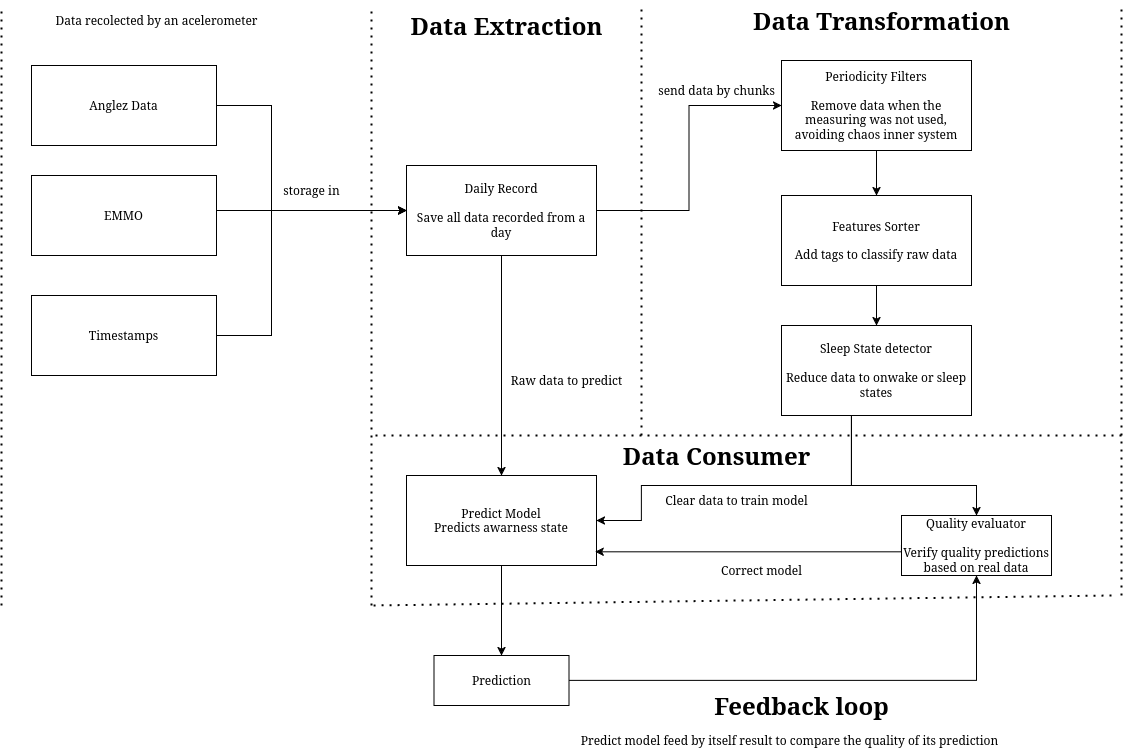
\includegraphics[width=\linewidth]{system.drawio(1).png}
    \caption{System Diagram}
\end{figure}
\subsection{System Engineering principles}
The system is architecure is designed taking into account a holistic view of the processing data flow and elements involved, divided by the following stages:
\begin{itemize}
	\item  \textbf{Data Extraction:} Environment entries are collected from the accelerometer, which is the main source of data for the system. The data is storage into chunks of one day.
	\item \textbf{Data Transformation:} Data is preprocessed to remove noise and irrelevant information by caothic filtering as unnecesary data from device removal periods. The data is then transformed into a format suitable for analysis, including feature extraction.
	\item \textbf{Data Consumer:} Data is consumed by stakeholders to define the sleep state between onwake or sleep. Along side, machine learning model is trained to detect sleep states based on the processed data. The model is evaluated and optimized in a feedback 
	loop which the outputs, predicitions made by the model, return to the system and verify how it is closed the model to the expected value.  
\end{itemize}

\end{document}